\chapter[Generalidades]{Generalidades sobre la marcha}

El siguiente capítulo pretende introducir al lector los conceptos fundamentales relacionados a la marcha y su estudio. Además de los avances tecnológicos en el área y el estado de estos.

\section{¿Qué es la marcha?}

Por \emph{marcha} se entiende el acto de desplazarse utilizando las extremidades corporales. Para \cite{perry} al caminar se utiliza una secuencia de movimientos de las extremidades, con el fin de mover el cuerpo hacia adelante y mantener la estabilidad. Cada una de estos ciclos (de la secuencia) involucra la interacción de dos extremidades inferiores, compuestas de varios segmentos, y la masa total del cuerpo. El estudio de la marcha consiste en la identificación de patrones de movimiento generados en la marcha y la segmentación del ciclo.

Es posible utilizar la física clásica para estudiar la marcha. Se puede describir la cinemática de la marcha al determinar las velocidades y aceleraciones de los segmentos rígidos del cuerpo; también se puede describir la dinámica de la marcha al determinar las fuerzas que actúan sobre los segmentos rígidos. Así, la marcha se estudia de dos maneras principales: el vector de fuerza recíproca generado por el suelo al soportar el peso del cuerpo y las velocidades de las principales uniones involucradas en la marcha. \citep{perry}

Ambas descripciones, cinemática y dinámica, se pueden utilizar para segmentar el ciclo de la marcha. \cite{perry} lo divide según muestra la tabla \ref{tab:ciclo_marcha}, donde se muestra de manera resumida, además la figura \ref{fig:ciclo_marcha} muestra imágenes tomadas del mismo autor. 

\begin{table}
    \centering
    \caption{Ciclo de la marcha según \cite{perry}}
    \label{tab:ciclo_marcha}
    \begin{tabular}{l l l}
        \toprule
        Función & Fase & Descripción \\
        \midrule
        Aceptación de la carga & Contacto Inicial & Justo cuando el pie toca el suelo \\
                               & Respuesta a la carga & El otro comienza el balanceo \\
        Soporte & Soporte medio & El centro de masa se alinea con el pié \\
                & Soporte final & El centro de masa sobrepasa el piel \\
        Avance del miembro & pre-balanceo & Se transfiere la carga al otro pie \\
                           & balanceo inicial & Se levanta el pie y avanza \\
                           & balanceo medio   & El pie sobrepasa al otro \\
                           & balanceo final   & Posición apta para contacto inicial \\
        \bottomrule
    \end{tabular}
\end{table}

\begin{figure}
    \centering
    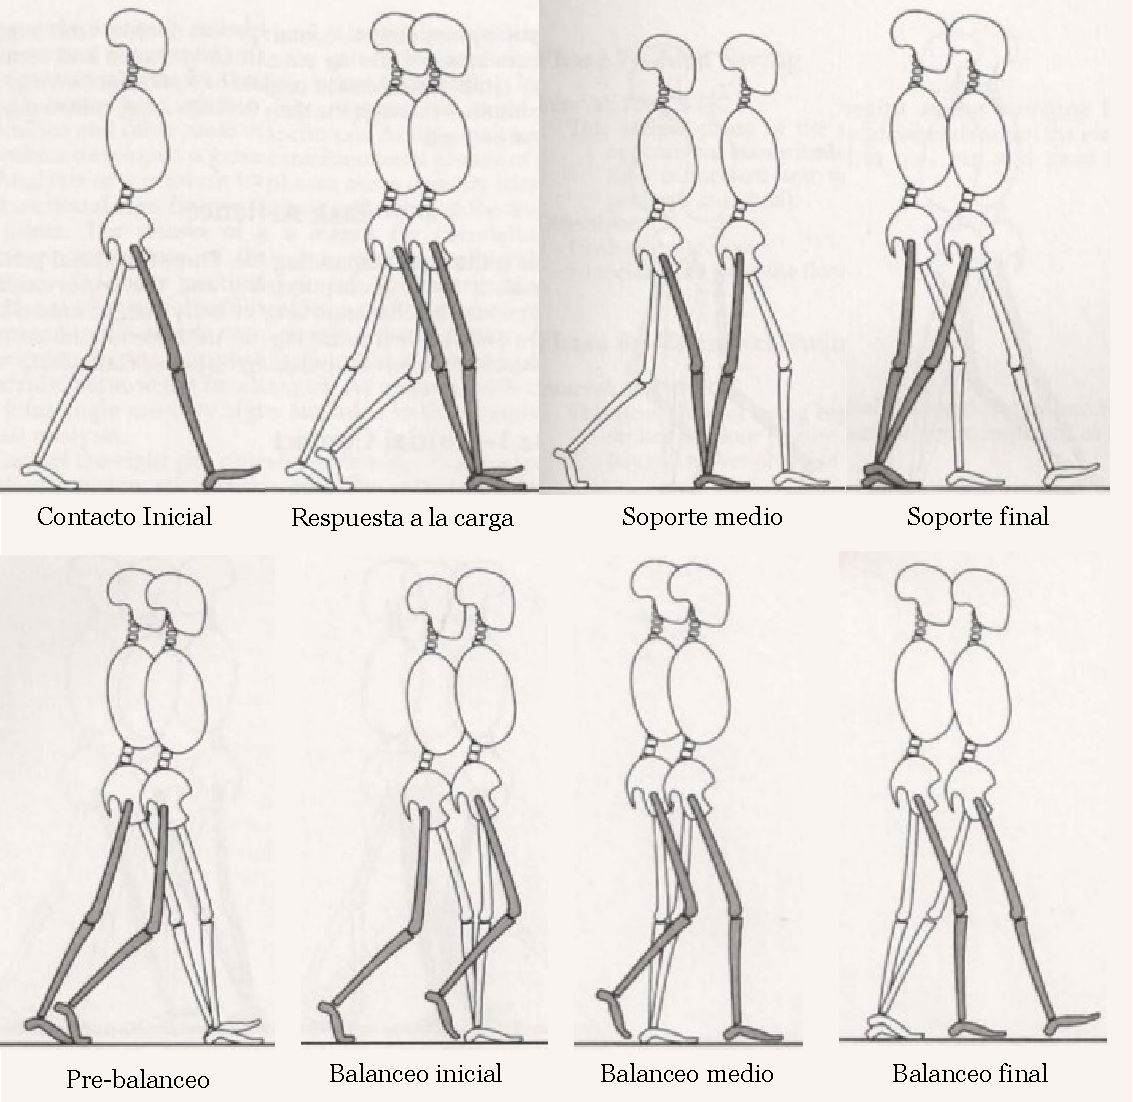
\includegraphics[width = \textwidth]{imagenes/ciclo_marcha}
    \caption{Ilustración del ciclo de la marcha, tomado de \citep{perry}}
    \label{fig:ciclo_marcha}
\end{figure}








\section[Herramient de diagnóstico]{Análisis de la marcha como herramienta de diagnóstico}

\section[Métodos de recolección]{Métodos de recolección de datos}

\section[Software disponible]{Software disponible para estudios sobre la marcha}
